% Options for packages loaded elsewhere
\PassOptionsToPackage{unicode}{hyperref}
\PassOptionsToPackage{hyphens}{url}
%
\documentclass[
]{article}
\usepackage{lmodern}
\usepackage{amssymb,amsmath}
\usepackage{ifxetex,ifluatex}
\ifnum 0\ifxetex 1\fi\ifluatex 1\fi=0 % if pdftex
  \usepackage[T1]{fontenc}
  \usepackage[utf8]{inputenc}
  \usepackage{textcomp} % provide euro and other symbols
\else % if luatex or xetex
  \usepackage{unicode-math}
  \defaultfontfeatures{Scale=MatchLowercase}
  \defaultfontfeatures[\rmfamily]{Ligatures=TeX,Scale=1}
\fi
% Use upquote if available, for straight quotes in verbatim environments
\IfFileExists{upquote.sty}{\usepackage{upquote}}{}
\IfFileExists{microtype.sty}{% use microtype if available
  \usepackage[]{microtype}
  \UseMicrotypeSet[protrusion]{basicmath} % disable protrusion for tt fonts
}{}
\makeatletter
\@ifundefined{KOMAClassName}{% if non-KOMA class
  \IfFileExists{parskip.sty}{%
    \usepackage{parskip}
  }{% else
    \setlength{\parindent}{0pt}
    \setlength{\parskip}{6pt plus 2pt minus 1pt}}
}{% if KOMA class
  \KOMAoptions{parskip=half}}
\makeatother
\usepackage{xcolor}
\IfFileExists{xurl.sty}{\usepackage{xurl}}{} % add URL line breaks if available
\IfFileExists{bookmark.sty}{\usepackage{bookmark}}{\usepackage{hyperref}}
\hypersetup{
  pdftitle={Working with Rmarkdown},
  pdfauthor={Matthew Toomey},
  hidelinks,
  pdfcreator={LaTeX via pandoc}}
\urlstyle{same} % disable monospaced font for URLs
\usepackage[margin=1in]{geometry}
\usepackage{color}
\usepackage{fancyvrb}
\newcommand{\VerbBar}{|}
\newcommand{\VERB}{\Verb[commandchars=\\\{\}]}
\DefineVerbatimEnvironment{Highlighting}{Verbatim}{commandchars=\\\{\}}
% Add ',fontsize=\small' for more characters per line
\usepackage{framed}
\definecolor{shadecolor}{RGB}{248,248,248}
\newenvironment{Shaded}{\begin{snugshade}}{\end{snugshade}}
\newcommand{\AlertTok}[1]{\textcolor[rgb]{0.94,0.16,0.16}{#1}}
\newcommand{\AnnotationTok}[1]{\textcolor[rgb]{0.56,0.35,0.01}{\textbf{\textit{#1}}}}
\newcommand{\AttributeTok}[1]{\textcolor[rgb]{0.77,0.63,0.00}{#1}}
\newcommand{\BaseNTok}[1]{\textcolor[rgb]{0.00,0.00,0.81}{#1}}
\newcommand{\BuiltInTok}[1]{#1}
\newcommand{\CharTok}[1]{\textcolor[rgb]{0.31,0.60,0.02}{#1}}
\newcommand{\CommentTok}[1]{\textcolor[rgb]{0.56,0.35,0.01}{\textit{#1}}}
\newcommand{\CommentVarTok}[1]{\textcolor[rgb]{0.56,0.35,0.01}{\textbf{\textit{#1}}}}
\newcommand{\ConstantTok}[1]{\textcolor[rgb]{0.00,0.00,0.00}{#1}}
\newcommand{\ControlFlowTok}[1]{\textcolor[rgb]{0.13,0.29,0.53}{\textbf{#1}}}
\newcommand{\DataTypeTok}[1]{\textcolor[rgb]{0.13,0.29,0.53}{#1}}
\newcommand{\DecValTok}[1]{\textcolor[rgb]{0.00,0.00,0.81}{#1}}
\newcommand{\DocumentationTok}[1]{\textcolor[rgb]{0.56,0.35,0.01}{\textbf{\textit{#1}}}}
\newcommand{\ErrorTok}[1]{\textcolor[rgb]{0.64,0.00,0.00}{\textbf{#1}}}
\newcommand{\ExtensionTok}[1]{#1}
\newcommand{\FloatTok}[1]{\textcolor[rgb]{0.00,0.00,0.81}{#1}}
\newcommand{\FunctionTok}[1]{\textcolor[rgb]{0.00,0.00,0.00}{#1}}
\newcommand{\ImportTok}[1]{#1}
\newcommand{\InformationTok}[1]{\textcolor[rgb]{0.56,0.35,0.01}{\textbf{\textit{#1}}}}
\newcommand{\KeywordTok}[1]{\textcolor[rgb]{0.13,0.29,0.53}{\textbf{#1}}}
\newcommand{\NormalTok}[1]{#1}
\newcommand{\OperatorTok}[1]{\textcolor[rgb]{0.81,0.36,0.00}{\textbf{#1}}}
\newcommand{\OtherTok}[1]{\textcolor[rgb]{0.56,0.35,0.01}{#1}}
\newcommand{\PreprocessorTok}[1]{\textcolor[rgb]{0.56,0.35,0.01}{\textit{#1}}}
\newcommand{\RegionMarkerTok}[1]{#1}
\newcommand{\SpecialCharTok}[1]{\textcolor[rgb]{0.00,0.00,0.00}{#1}}
\newcommand{\SpecialStringTok}[1]{\textcolor[rgb]{0.31,0.60,0.02}{#1}}
\newcommand{\StringTok}[1]{\textcolor[rgb]{0.31,0.60,0.02}{#1}}
\newcommand{\VariableTok}[1]{\textcolor[rgb]{0.00,0.00,0.00}{#1}}
\newcommand{\VerbatimStringTok}[1]{\textcolor[rgb]{0.31,0.60,0.02}{#1}}
\newcommand{\WarningTok}[1]{\textcolor[rgb]{0.56,0.35,0.01}{\textbf{\textit{#1}}}}
\usepackage{longtable,booktabs}
% Correct order of tables after \paragraph or \subparagraph
\usepackage{etoolbox}
\makeatletter
\patchcmd\longtable{\par}{\if@noskipsec\mbox{}\fi\par}{}{}
\makeatother
% Allow footnotes in longtable head/foot
\IfFileExists{footnotehyper.sty}{\usepackage{footnotehyper}}{\usepackage{footnote}}
\makesavenoteenv{longtable}
\usepackage{graphicx,grffile}
\makeatletter
\def\maxwidth{\ifdim\Gin@nat@width>\linewidth\linewidth\else\Gin@nat@width\fi}
\def\maxheight{\ifdim\Gin@nat@height>\textheight\textheight\else\Gin@nat@height\fi}
\makeatother
% Scale images if necessary, so that they will not overflow the page
% margins by default, and it is still possible to overwrite the defaults
% using explicit options in \includegraphics[width, height, ...]{}
\setkeys{Gin}{width=\maxwidth,height=\maxheight,keepaspectratio}
% Set default figure placement to htbp
\makeatletter
\def\fps@figure{htbp}
\makeatother
\setlength{\emergencystretch}{3em} % prevent overfull lines
\providecommand{\tightlist}{%
  \setlength{\itemsep}{0pt}\setlength{\parskip}{0pt}}
\setcounter{secnumdepth}{-\maxdimen} % remove section numbering

\title{Working with Rmarkdown}
\author{Matthew Toomey}
\date{8/14/2022}

\begin{document}
\maketitle

\begin{center}\rule{0.5\linewidth}{0.5pt}\end{center}

\hypertarget{introduction}{%
\section{Introduction}\label{introduction}}

Rmarkdown is a valuable tool to organize code, comments, and output for
communication and archiving. I encourage you to use this format to work
through our lessons and take notes.

Here we will walk through the basics of Rmarkdown. A helpful quick
references is available in Rstudio
\texttt{Help\ \textgreater{}\ Markdown\ Quick\ Reference}:

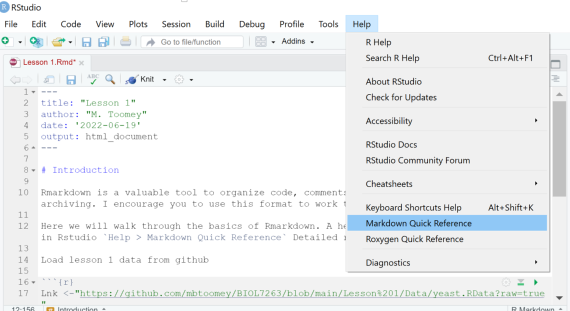
\includegraphics{Help.PNG}

A more detailed reference is available at the
\href{https://bookdown.org/yihui/rmarkdown-cookbook/}{rmarkdown
cookbook}.

\hypertarget{file-types}{%
\subsubsection{File types}\label{file-types}}

\begin{itemize}
\tightlist
\item
  \texttt{.Rmd} is Rstudio's secific formulation of Markdown (a text
  rendering language)
\item
  \texttt{.md} is the more generic Markdown file type. In RStudio, the
  intermediate \texttt{.md} files are not (in the default state)
  preserved.This is the format of your ``readme'' file on GitHub.
\end{itemize}

\hypertarget{basic-text-formatting}{%
\subsubsection{Basic text formatting}\label{basic-text-formatting}}

\begin{itemize}
\tightlist
\item
  headers \texttt{\#} to \texttt{\#\#\#\#\#\#} *numbering from options
\item
  text
\item
  markup

  \begin{itemize}
  \tightlist
  \item
    italic \texttt{*\textless{}text\textgreater{}*}
  \item
    bold-face \texttt{**\textless{}text\textgreater{}**}
  \item
    subscript
    \texttt{\textasciitilde{}\textless{}text\textgreater{}\textasciitilde{}}
  \item
    superscript \texttt{\^{}\textless{}text\textgreater{}\^{}}
  \item
    strikethrough
    \texttt{\textasciitilde{}\textasciitilde{}\textless{}text\textgreater{}\textasciitilde{}\textasciitilde{}}
  \item
    quotations
    \texttt{\textgreater{}\textless{}text\ with\ no\ closing\ mark}
  \end{itemize}
\end{itemize}

\hypertarget{spacing-manual-breaks-lines}{%
\subsubsection{Spacing, manual breaks,
lines}\label{spacing-manual-breaks-lines}}

\begin{itemize}
\tightlist
\item
  line spacing effects
\item
  two extra spaces at the end of a line for a manual break
\item
  lists

  \begin{itemize}
  \tightlist
  \item
    indented
  \item
    numbered
  \end{itemize}
\end{itemize}

\hypertarget{insert-links-and-images}{%
\subsubsection{Insert links and images}\label{insert-links-and-images}}

\begin{itemize}
\tightlist
\item
  links
\end{itemize}

\begin{verbatim}
[Dr. Toomey's website](http://mbtoomey.net)
\end{verbatim}

\href{http://mbtoomey.net}{Dr.~Toomey's website}

\begin{itemize}
\tightlist
\item
  images
\end{itemize}

\begin{verbatim}
![Peanguin](Penguin.jpg)
\end{verbatim}

\begin{figure}
\centering
\includegraphics{Penguin.jpg}
\caption{Peanguin}
\end{figure}

\hypertarget{lists}{%
\subsubsection{Lists}\label{lists}}

\hypertarget{lists-1}{%
\section{Lists}\label{lists-1}}

\hypertarget{unordered-list}{%
\subsection{unordered list}\label{unordered-list}}

\begin{verbatim}
- Finches
- Sparrows
    - House sparrow
    - Tree sparrow
\end{verbatim}

For second level list items ``-'' is preceeded by two spaces

\begin{itemize}
\tightlist
\item
  Finches
\item
  Sparrows

  \begin{itemize}
  \tightlist
  \item
    House sparrow
  \item
    Tree sparrow
  \end{itemize}
\end{itemize}

\hypertarget{order-lists}{%
\subsection{Order lists}\label{order-lists}}

\begin{verbatim}
1. Finches
2. Sparrows
    - House sparrow
    - Tree sparrow
\end{verbatim}

\begin{enumerate}
\def\labelenumi{\arabic{enumi}.}
\tightlist
\item
  Finches
\item
  Sparrows

  \begin{itemize}
  \tightlist
  \item
    House sparrow
  \item
    Tree sparrow
  \end{itemize}
\end{enumerate}

\hypertarget{fencing}{%
\section{Fencing}\label{fencing}}

\begin{verbatim}
Anything surrounded by backticks `will render as plain text` 
\end{verbatim}

Anything surrounded by backticks \texttt{will\ render\ as\ plain\ text}

\begin{Shaded}
\begin{Highlighting}[]
\NormalTok{R code inside ticks can be executed during rendering. For example, you can caluclate a value }\StringTok{`}\DataTypeTok{r 3 + pi}\StringTok{`}\NormalTok{. }
\end{Highlighting}
\end{Shaded}

R code inside ticks can be executed during rendering. For example, you
can caluclate a value 6.1415927.

You can create a whole block of plain text by surrounding it with three
backticks

\begin{verbatim}
everything is plain text here.
even single lines

Useful for show blocks of codes
\end{verbatim}

\hypertarget{block-quotes-with}{%
\section{\texorpdfstring{Block quotes with
\texttt{\textgreater{}}}{Block quotes with \textgreater{}}}\label{block-quotes-with}}

\begin{verbatim}
> Whether I shall turn out to be the hero of my own life, or whether that station will be held by anybody else, these pages must show.
\end{verbatim}

\begin{quote}
Whether I shall turn out to be the hero of my own life, or whether that
station will be held by anybody else, these pages must show.
\end{quote}

\hypertarget{spacer-line-with-three-or-more-underscores}{%
\section{Spacer line with three or more
underscores}\label{spacer-line-with-three-or-more-underscores}}

\begin{verbatim}
___   
\end{verbatim}

\begin{center}\rule{0.5\linewidth}{0.5pt}\end{center}

\hypertarget{tables}{%
\section{Tables}\label{tables}}

\begin{verbatim}
| Species  | Awesomeness
| :------------- | :-------------
| House Sparrow   | Medium|
| Tree Sparrow  | High|
\end{verbatim}

\begin{longtable}[]{@{}ll@{}}
\toprule
Species & Awesomeness\tabularnewline
\midrule
\endhead
House Sparrow & Medium\tabularnewline
Tree Sparrow & High\tabularnewline
\bottomrule
\end{longtable}

The ``-'' set the width of column The ``:'' set the justification

\hypertarget{equations}{%
\subsubsection{Equations}\label{equations}}

\begin{itemize}
\item
  in-line \texttt{\$}
\item
  centered \texttt{\$\$}
\item
  basic math and text spacing handled by LateX. Note that this language
  is a bit different than the basic markdown (e.g.~how sub and
  superscripts are handled)
\end{itemize}

\begin{verbatim}
$$y = a + b$$
\end{verbatim}

\[y = a + b\]

\hypertarget{subcripts}{%
\paragraph{Subcripts}\label{subcripts}}

\begin{verbatim}
$$H_0 = Z_{a + b}$$
\end{verbatim}

\[H_0 = Z_{a + b}\]

\hypertarget{superscripts}{%
\paragraph{Superscripts}\label{superscripts}}

\begin{verbatim}
$$S = cA^z$$
\end{verbatim}

\[S = cA^z\]

\begin{itemize}
\tightlist
\item
  elements can be coupled and nested
\end{itemize}

\[S=cA^z_1 + z_{2 + x}\]

\begin{verbatim}
$$S=cA^z_1 + z_{2 + x}$$
\end{verbatim}

\hypertarget{fractions-and-greek-symbols}{%
\paragraph{Fractions and Greek
Symbols}\label{fractions-and-greek-symbols}}

\[\alpha = \frac{\beta}{\delta + \gamma_x}\]

\begin{verbatim}
$$\alpha = \frac{\beta}{\delta + \gamma_x}$$
\end{verbatim}

\hypertarget{summation-signs}{%
\paragraph{Summation signs}\label{summation-signs}}

\[z = \sum_{i=1}^X{K}\]

\begin{verbatim}
$$z = \sum_{i=1}^X{K}$$
\end{verbatim}

\hypertarget{what-is-you-need-a-backslash-in-your-equation}{%
\paragraph{What is you need a backslash in your
equation?}\label{what-is-you-need-a-backslash-in-your-equation}}

Use \texttt{\textbackslash{}backslash}

\begin{verbatim}
$$\backslash \alpha \le b \backslash$$
\end{verbatim}

\[\backslash \alpha \le b \backslash\]

\hypertarget{rendering-plain-text-in-a-latex-equation}{%
\paragraph{Rendering plain text in a LaTex
Equation}\label{rendering-plain-text-in-a-latex-equation}}

\[P(Expression of gene) = Z\]

\begin{verbatim}
$$P(Expression of gene) = Z$$
\end{verbatim}

\[P(\mbox{Expression of gene}) = Z\]

\begin{verbatim}
$$P(\mbox{Expression of gene}) = Z$$
\end{verbatim}

\end{document}
